\section{Spacecraft Deign Overview}
Summarised in table~\ref{tab:designoverview} below is the outline of all components in the SnapSat proposed design.

\begin{table}[H]
    \centering
    \caption{SnapSat Design Overview}
    \vspace{0.15cm}
    \label{tab:designoverview}
    {\renewcommand{\arraystretch}{1.4}%
        \begin{tabular}{|>{\arraybackslash}m{3cm}|>{\arraybackslash}m{10cm}|}
            \hline
            \textbf{Subsystem} & \textbf{Description} \\ \hline\hline
            Structural & - industrial grade aluminium \newline - laser cut, bent to shape and riveted together \\\hline
            ADCS & - air core magneto-torquers made in-house \newline - Osram SFH203P Photodiodes \newline - IMU: Adafruit 9-DOF  \\\hline
            EPS & - Australian Robotics solar panels \newline - battery: LiNiMnCo 26650 rechargeable cell  \\\hline
            OBC / OBDH & - Arduino DUE \newline - 4 $\times$ PCBs (power, control, EPS and communications)  \\\hline
           TT\&C & - VHF (Xbee) \newline - UHF \newline - tape measure antennae \\\hline
           Thermal & - thermal tapings and passive coatings (Kapton tape) \newline - selected components will have multi-layer insulation \\\hline
           Payload & - Arducam \\\hline
        \end{tabular} } 
    \end{table}
    
\subsection{Subsystem Design Schematic}
The layout of Snapsat, with the interconnects of power and data lines between the subsystems is shown in the figure below.The Solar panels will be arranged according to Figure~\ref{fig:flower}.  This design has been chosen to maximize the solar panel area of the SnapSat while still abiding by the volume/size limitations of CubeSats.  Increasing the solar panel area has given us the ability to power a higher quality camera, increasing the performance of the payload and usefulness of the SnapSat.

\begin{figure}[H]
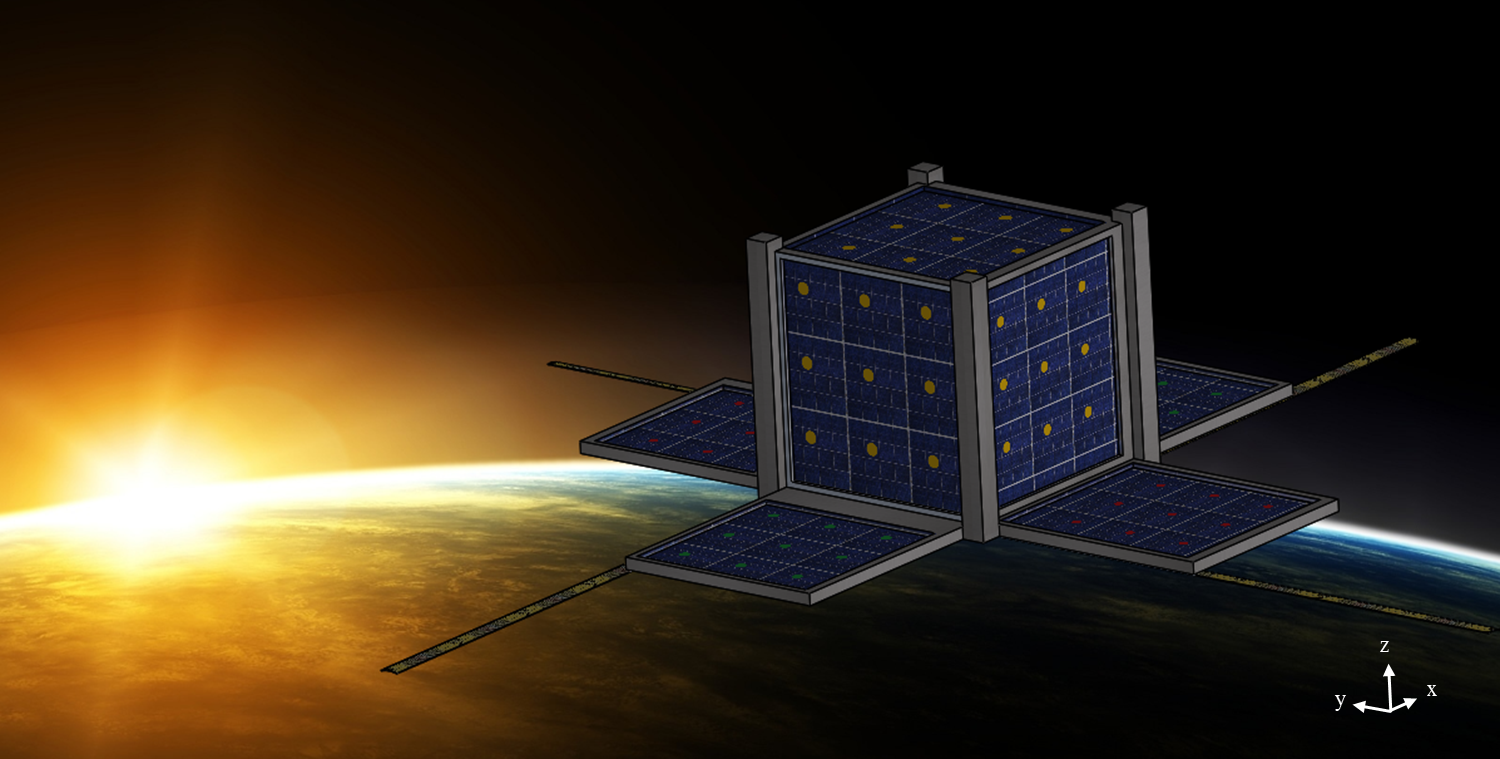
\includegraphics[width=\textwidth]{Picture1}
\caption{Design Schematic for SnapSat - the colours indicated the panels that power the batteries. There are three individual batters and so three sets of solar panels to power them}
\label{fig:flower}
\end{figure}
\noindent
In the following report yaw will be refereed to as rotation about the z axis, roll about the x axis and pitch about the y axis (although these are relatively interchangeable as the SnapSat is rotationally almost symmetric). The flow chart describing how the system integrates is shown over the page.

\begin{figure}[H]
    \pic{1}{flow2}{Design Schematic}
\end{figure}
